\section{Software architecture}
\label{architecture}

The EASAL software has two versions. The TOMS submission contains only the
backend of EASAL, without GUI and with text input and output.  An optional GUI
(not part of TOMS submission) which can be used for intuitive visual
verification of the results, can be found at the EASAL bitbucket repository
\cite{easalSoftware}. \figref{fig:Architecture}, which shows the overall
architecture of EASAL, clearly demarcates these two versions.

The user initiates the sampling either by running just the backend in a
terminal or through the optional GUI (not part of TOMS submission). The
AtlasBuilder starts the sampling process by making a recursive call to the
`sampleAtlasNode' algorithm with the root node as the parameter. The Atlas
builder interacts with various components such as `Cayley parameterization',
`Cartesian Realization' and `Constraint Check' to help in the sampling process.
It uses the `SaveLoader' to save the generated atlas to the database.  All the
sampling information such as the atlas, active constraint graphs, Cayley
parameters and realizations are written to a database to avoid re-sampling.

When EASAL is initiated using the backend, the output is in text format.
The following are the output:
\begin{itemize}
\item The \emph{Roadmap}, which stores the atlas, i.e., a topologically
stratified set of sample feasible realizations or configurations of the two
rigid point sets. This can be found in the `RoadMap.txt' file in the data
folder.

\item The \emph{Node} files which contain sampling information, Cayley
parameter values, and realizations of the point sets. Each `Node*.txt' file
contains samples for a particular active constraint region.

\item The \emph{paths} file which contains the one degree of freedom motion
path between all pairs of lowest energy configuration regions. This can be
found in the `paths.txt' file in the data folder.

\item The \emph{path matrix}, which contains a path matrix where the rows and
columns correspond to 0D and 1D nodes. The $\{ij\}^{th}$ entry indicates the
number of paths between nodes $i$ and $j$. This can be found in the
`path\_matrix.txt' file in the data folder.
\end{itemize}

The optional GUI (not part of TOMS submission) can be used to visualize the
output of the backend. See Section 3.3.5 of the `Complete User Guide' located
in the bitbucket repository \cite{easalSoftware} for instructions.  The
optional GUI has three views: the \emph{atlas view}, the \emph{Cayley space
view} and the \emph{realization view}.  The atlas view shows the stratification
of the configuration space in the form of an atlas. In the atlas view, the user
can explore the atlas by intervening in the sampling process to either
complete, redirect, refine or limit the sampling.  The user can also propose
new constraints for active constraint graphs.  The Cayley space view shows the
user the Cayley configuration space of a node in the atlas.  In the Cayley
space view the user can view all the Cayley parameters and boundaries. In the
realization view, the user can view all the Cartesian realizations of the
selected node.  This view contains the \emph{sweep} feature which keeps one of
the point-sets fixed and draws the other point-set many times to trace out the
set of all feasible realizations. 


\begin{figure}
\centering
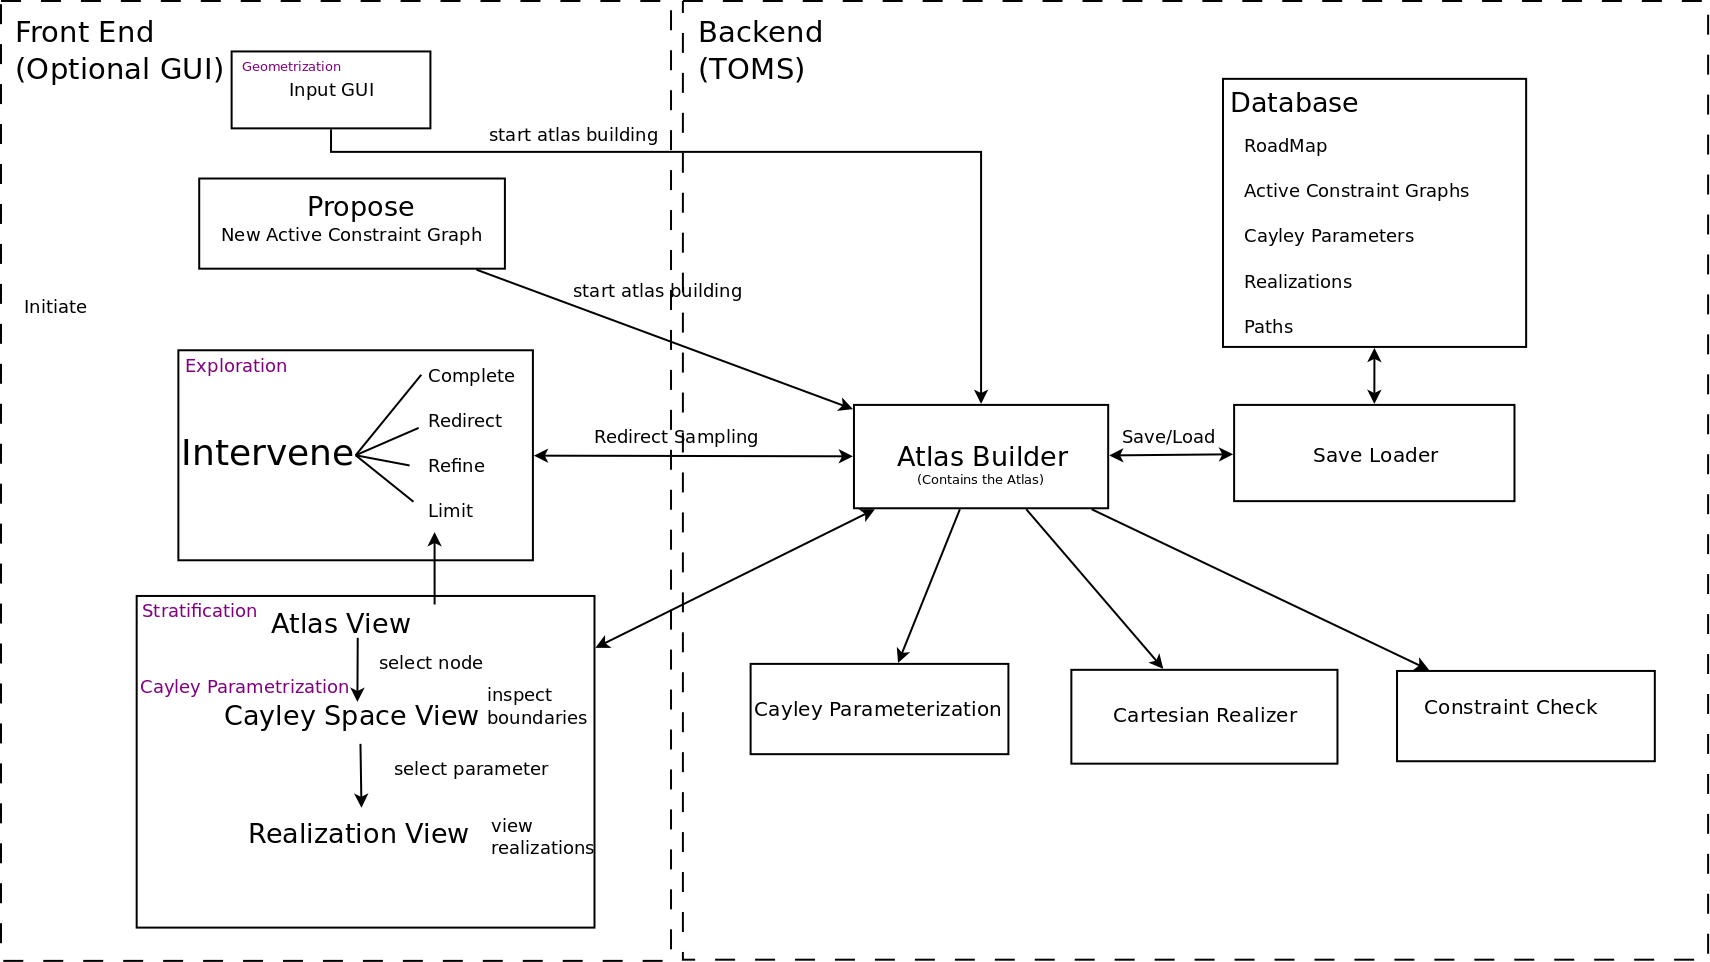
\includegraphics[width=\textwidth] {\fig/Architecture.png}
\caption{Architecture of \EASAL.}
\label{fig:Architecture}
\end{figure}
